\documentclass[11pt]{article}
\usepackage[dvipsnames]{xcolor}
% Packages
\usepackage{amsmath, amsthm, amssymb}
\usepackage{hyperref}
\usepackage{graphicx}
\usepackage{tikz}
\usetikzlibrary{calc,positioning}
\usetikzlibrary{shapes.multipart}
\usepackage[utf8]{inputenc}
\usepackage[linesnumbered,vlined,ruled]{algorithm2e}
\SetCommentSty{emph}
\SetKwProg{Fn}{\textbf{Function}}{}{}
\usepackage{geometry}
\usepackage{mdframed}
\usepackage{tikz-qtree}


\usepackage{enumitem}
\usepackage{mdframed}
\usepackage{subcaption}
\usepackage[capitalize,noabbrev]{cleveref}

\newcommand{\PRF}{\ensuremath{{\sf PRF}}}
\newcommand{\FHE}{\ensuremath{{\sf FHE}}}
\newcommand{\Gen}{\ensuremath{{\sf Gen}}}
\newcommand{\Eval}{\ensuremath{{\sf Eval}}}
\newcommand{\Enc}{\ensuremath{{\sf Enc}}}
\newcommand{\Dec}{\ensuremath{{\sf Dec}}}
\newcommand{\Seed}{\ensuremath{{\sf Seed}}}
\newcommand{\DB}{\ensuremath{{\sf DB}}}
\newcommand{\Comm}{\ensuremath{{\sf Comm}}}
\newcommand{\xor}{\ensuremath{\oplus}}
\newcommand{\Sim}{\ensuremath{{\sf Sim}}}
\newcommand{\negl}{\ensuremath{{\sf negl}}}
\newcommand{\sk}{\ensuremath{{\sf sk}}\xspace}
\newcommand{\pk}{\ensuremath{{\sf pk}}\xspace}
\newcommand{\ignore}[1]{}
\newcommand{\key}{\ensuremath{{\sf key}}}
\newcommand{\getr}{\ensuremath{~{\overset{\$}{\leftarrow}}}~}

\newcommand{\elaine}[1]{{\color{red} [elaine: #1]}}
\newcommand{\mingxun}[1]{{\color{red} [mz: #1]}}

\definecolor{darkgreen}{RGB}{34, 139, 34}
\definecolor{darkred}{rgb}{0.5, 0, 0}
\definecolor{lightblue}{RGB}{0,176,240}



\definecolor{g1}{gray}{0.7}
\definecolor{g2}{gray}{0.6}
\definecolor{g3}{gray}{0.5}
\definecolor{g4}{gray}{0.4}
\definecolor{g5}{gray}{0.3}
\definecolor{g6}{gray}{0.2}
\definecolor{g7}{gray}{0.1}
\definecolor{g8}{gray}{0}



\geometry{a4paper, margin=1in}

\theoremstyle{definition}
% Theorem Environments
\newtheorem{theorem}{Theorem}
\newtheorem{remark}{Remark}
\newtheorem{lemma}[theorem]{Lemma}
\newtheorem{corollary}[theorem]{Corollary}
\newtheorem{definition}[theorem]{Definition}
\newtheorem{proposition}[theorem]{Proposition}
\newtheorem{claim}[theorem]{Claim}


% Document Informatio n
\title{{\Large Cryptography Meets Algorithms (15893) Lecture Notes}\\[5pt]
{\bf Lecture 11: ORAM Lower Bound}}
\author{Scribe: Kunming Jiang}
\date{\today}

\begin{document}

\maketitle

% Please create a file named noteX.tex, where X is the number of the course. 
% Only edit the noteX.tex if possible.
% If you want to define macros, please have them inside the noteX.tex file.

{
%\usepackage{xspace}

\newcommand{\bits}{\{0,1\}}
\newcommand{\bfu}{\mathbf{u}}
\newcommand{\bfv}{\mathbf{v}}
\newcommand{\bfp}{\mathbf{p}}
\newcommand{\bfz}{\mathbf{z}}
\newcommand{\bfx}{\mathbf{x}}
\newcommand{\bfy}{\mathbf{y}}

\newcommand{\calR}{\mathcal{R}}

\newcommand{\CNextMsg}{\ensuremath{{\sf C Next Msg}}}
\newcommand{\SNextMsg}{\ensuremath{{\sf S Next Msg}}}
\newcommand{\CNext}{\ensuremath{{\sf C Next}}}
\newcommand{\SNext}{\ensuremath{{\sf S Next}}}
\newcommand{\Cstp}{\ensuremath{{\sf Cst'}}}
\newcommand{\Cst}{\ensuremath{{\sf Cst}}}
\newcommand{\msg}{\ensuremath{{\sf msg}}}
\newcommand{\msgp}{\ensuremath{{\sf msg'}}}
\newcommand{\Coutput}{\ensuremath{{\sf Reconstr}}}
\newcommand{\ans}{\ensuremath{{\sf ans}}}
\newcommand{\Ccoins}{\ensuremath{{\sf Ccoins}}}
\newcommand{\Scoins}{\ensuremath{{\sf Scoins}}}
\newcommand{\Expt}{\ensuremath{{\sf Expt}}}
\newcommand{\coin}{\ensuremath{{\sf coin}}}
\newcommand{\View}{\ensuremath{{\sf View}}}
\newcommand{\PPT}{PPT }
\newcommand{\Out}{\ensuremath{{\sf Out}}}
\newcommand{\OWF}{\ensuremath{{\sf OWF}}}
\newcommand{\OT}{\ensuremath{{\sf OT}}}
\newcommand{\PIR}{\ensuremath{{\sf PIR}}}
\newcommand{\Server}{\ensuremath{{\sf Server}}}
\newcommand{\Client}{\ensuremath{{\sf Client}}}
\newcommand{\Alice}{\ensuremath{{\sf Alice}}}
\newcommand{\Bob}{\ensuremath{{\sf Bob}}}
\newcommand{\get}{\ensuremath{\leftarrow}}
\newcommand{\E}{\ensuremath{{\bf E}}}
\newcommand{\out}{\ensuremath{{\sf out}}}
\newcommand{\addr}{\vec{\mbox{addr}}}
\newcommand{\action}{\vec{\mbox{action}}}
\newcommand{\op}{\vec{\mbox{op}}}
\newcommand{\mread}{\mbox{read}}
\newcommand{\mwrite}{\mbox{write}}

\newcommand{\red}[1]{{}\color{red}#1}

\tikzset{every tree node/.style={minimum width=2em,draw},
         blank/.style={draw=none},
         edge from parent/.style=
         {draw,edge from parent path={(\tikzparentnode) -- (\tikzchildnode)}},
         level distance=1.5cm}

In this lecture, we will prove that any Oblivious RAM (ORAM)
scheme must suffer from logarithmic overhead. 
We will show two proofs.  The first
proof was 
described in Goldreich and Ostrovsky's original paper on 
ORAM~\cite{goldreich96software}. 
Their lower bound has two restrictions: 
1) it works only for {\it statistically} secure ORAMs and 
2) 
it assumes that the ORAM is in the {\it balls-and-bins}
model, i.e., the scheme does not perform
any encoding on the payload strings stored in memory.
Many years later, in 2018, the 
work of Larsen and Nielsen~\cite{larsen18lowerbound}
proved a new lower bound removing both of these restrictions. 
Interestingly, their proof uses techniques
from the data structure lower bound literature.
We will also 
cover Larsen and Nielsen's lower bound in today's lecture.




\section{Goldreich and Ostrovsky's Lower Bound}

\begin{theorem}
Consider any perfectly secure ORAM scheme in the balls-and-bins model
such that the ORAM begins with 
a memory already loaded with $n$ words. 
Then, any 
logical request sequence of length $t$ 
must incur $\max(n, \Omega(t \log t))$ total cost. 
Further, the lower bound works even for read-only 
requests. 
\end{theorem}
\begin{proof}
Consider the following game. 
Initially, there are $n$ balls, and ball $i$ is stored in cell $i$
of the memory.
There is a sequence of $t$ logical requests, to read
the balls indexed $i_1, \ldots, i_t$ respectively.
A player 
can hold up to $m$ balls in her hand. 
In every time step indexed $1, 2, \ldots, q$, she 
can visit a memory cell of her choice and 
perform one of the following hidden operations:
\begin{enumerate}[itemsep=1pt]
\item 
Take a ball from the memory cell and put it in her hand;
\item 
Place a ball from her hand to the memory cell (if it is currently empty);
\item 
Do nothing.
\end{enumerate}
The player's action sequence 
can satisfy the request sequence, iff there is  
a subsequence 
$1\leq j_1 \leq j_2 \leq \ldots \leq j_t \leq q$, such
that for all $k \in [t]$, 
the ball indexed $i_k$ is in the player's hands
at the end of 
time step $j_k$. 

Suppose that an adversary can observe which memory cell
the player visits in every time step,  
but cannot observe which hidden operation the player performs. 
Similarly, the adversary cannot observe which balls are 
stored in the memory cells or the player's hands.
Now, the player's job is to satisfy the logical request
sequence $i_1, \ldots, i_t$ without revealing any information 
about the logical request sequence.
\end{proof}


\textbf{Goldreich-Ostrovsky Lower Bound \cite{goldreich96software}} Any ORAM scheme (in the balls-and-bins model) must have at least logarithmic overhead. 

\noindent To prove, let
\begin{itemize}
  \item $m =$ number of balls the client can hold in its hand
  \item $t =$ logical request sequence length
  \item $n =$ memory size
\end{itemize}

\noindent Every step, client can visit some memory location $i$, and
\begin{enumerate}
  \item take no action
  \item take a ball from $i$
  \item place a ball into $i$
\end{enumerate}

\noindent Now given
\begin{itemize}
  \item initial memory with $n$ balls,
  \item requests $r_1\dots r_t$
  \item implementation $(\addr, \action)$ and $q = |\addr|$
\end{itemize}
an observer can only see $\addr$ but not $\action$.

\bigskip
\noindent\emph{Q: Assume perfect security, how many request sequences can $\addr$ realize?}
\begin{enumerate}
  \item For every request, there are $m+2$ possible action (1 from doing nothing, 1 from taking a ball, and $m$ from placing a ball).
  \item At the end of each $(\addr, \action)$, the client can use the $m$ balls it has to express $m$ different results.
  \item Need to realize all $n^t$ possible memory access sequences.
\end{enumerate}
Thus,
$$
\begin{array}{rcl}
  (m+2)^q \cdot m^q \geq n^t & \Rightarrow & q\log m + q\log(m+2) \geq t\log n \\
  & \Rightarrow & q/t \geq \frac{\log n}{2\log (m+2)}
\end{array}
$$

\noindent Restrction of G-O LB:
\begin{enumerate}
  \item Balls and bins assumptions
  \item Only works for statistically secure schemes
\end{enumerate}

\section{Lauren-Nielsen}

\textbf{Lauren-Nielsen Lower Bound \cite{larsen18lowerbound}} Logarithmic LB for ORAM but removing these restrictions.

\noindent Assumptions:
\begin{itemize}
  \item read and write in ``word''
  \item word size $\geq \log N$ (memory size)
\end{itemize}

Assume that there is a binary tree, where each leaf node corresponds to a consecutive (read, write) pair. W.L.o.G, fix 
$$\op = \mread(0), \mwrite(0, 0), \dots, \mread(0), \mwrite(0, 0)$$
Want to show: number of probes into memory must be "high" for $\op$.

\noindent \emph{How the tree helps us count}: suppose $\mbox{op}_j$ probes some mem location, and the last time this location was probed was during $\mbox{op}_i$. Then we charge this probe to the least common ancestor in the tree of $\mbox{op}_i$ and $\mbox{op}_j$.

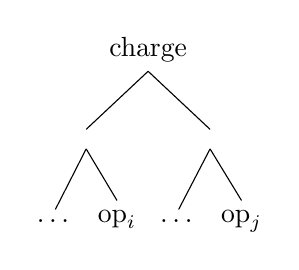
\begin{tikzpicture}
  \Tree
  [.\red{charge}     
      [.{} 
        [.{\dots} ]
        [.\red{$\mbox{op}_i$} ]
      ]
      [.{}
        [.{\dots} ]
        [.\red{$\mbox{op}_j$} ]
      ]
  ]
\end{tikzpicture}

Assume that the adversary can observe the physical probe locations and the boundary between each $\mbox{op}$. Then it can construct this tree in polynomial time, i.e. how many probes are charged to each node. (\emph{This is where computational security kicks in.})

By ORAM security: $\forall\ \op, \op'$ of same length, the two trees constructed must be computationally indistinguishable from each other.

For every subtree $v$ of size $2m$, let the left half of the leaves denote
$$\mread(0), \mwrite(1, r_1)$$
$$\vdots$$
$$\mread(0), \mwrite(m, r_m)$$
and the right half denote
$$(\mread(1), \mwrite(0, 0))$$
$$\vdots$$
$$(\mread(m), \mwrite(0, 0))$$

Idea: when we count the probes assigned to each node $v$, we can use the worst-case sequence for $v$.

Intuition: imagine balls-and-bins model, number of probes assigned to $v \geq\frac{|\mbox{leaves under } v|}{2}$. Thus, at each level, there will be at least $T/2$ probes. Since there are $\log T$ levels, total number of probes at least $O(T \log T)$.

\textbf{Information Transfer Technique} (Encoding Argument): let coins be the randomness consumed by ORAM.
\begin{itemize}
  \item Encode ($r_1, \dots r_m$, coins)
  \begin{enumerate}
    \item Execute ORAM over prefix $\mread(0), \mwrite(0, 0), \dots$
    \item Execute $\mread(0), \mwrite(1, r_1), \dots, \mread(0), \mwrite(m, r_m)$
    \item Execute $\mread(1), \mwrite(0, 0), \dots, \mread(m), \mwrite(0, 0)$
  \end{enumerate}
  \item Encoding ($C$) = for each memory location probed during 2 and 3, record (location, last value written during 2) and the CPU register at the end of 2
  \item Decode ($C$, coins)
  \begin{enumerate}
    \item Same as 1 in Encode
    \item Reset CPU state to $C$.cpuState for every (loc, val) in $C$, let mem[loc]$\leftarrow$ val
    \item same as 3 in Encode
  \end{enumerate}
  \item Decoder output the outcomes of the read ops in 3
\end{itemize}


}
%{
%\newcommand{\bits}{\{0,1\}}
\newcommand{\bfu}{\mathbf{u}}
\newcommand{\bfv}{\mathbf{v}}
\newcommand{\bfp}{\mathbf{p}}
\newcommand{\bfz}{\mathbf{z}}
\newcommand{\bfx}{\mathbf{x}}
\newcommand{\bfy}{\mathbf{y}}

\newcommand{\bbZ}{\mathbb{Z}}
\newcommand{\calR}{\mathcal{R}}

\section{Sub-poly Communication 2-server Classical PIR}

As introduced in the earlier lecture, Private Information Retreival~(PIR)~\cite{chor1998private} is a cryptographic mechanism which allows a user holding an index $i\in[n]$ to retrieve the $i$-th bit from a $n$-bit database, copies of which are held by one or more (non-colluding) servers, such that the servers do not learn anything about about $i$. We saw a construction of two-server information-theoretic PIR that has bandwidth $O(n^{1/3})$ in the last lecture. The ultimate goal in this lecture is to see at a PIR construction that has bandwidth sub-polynomial in $n$.
As a first step, we will see a 2-server PIR construction by Woodruff and Yekhanin~\cite{woodruff2005geometric} that has bandwidth $O(n^{1/3})$, based on an interpolation approach.
\subsection{An Interpolation Approach to 2-Server PIR}
As a warm-up, we will first start with a na\"ive \emph{four-server} construction. Let $\bfx=(x_1,x_2,\ldots,x_n)\in \bits^n$ be the database. Define $E:[n]\to \bits^m$ such that $E(1),E(2),\ldots,E(n)$ are $n$ distinct points of Hamming weight $3$. Note that such a mapping $E$ exists as long as ${m\choose 3}\ge n$. Hence, we set $m=O(n^{1/3})$. Define the multivariate polynomial $F(z_1,z_2,\ldots,z_m)$ over $\mathbb{F}_5$ as
\[
F(z_1,z_2,\ldots,z_m)=\sum_{i=1}^nx_i\prod_{E(i)_\ell=1}z_\ell\;.
\]
First off, observe that since each $E(i)$ has hamming weight $3$, $F$ has degree $3$. Furthermore, for each $i$, $F(E(i))=x_i$.

Therefore, in the PIR protocol a user that has index $i$, needs to retrieve the value of $F(\bfp)$ for $\bfp=E(i)$. Let $\bfv$ be some randomly chosen element of $\mathbb{F}_5^m$. Suppose, the user learns the values $F(\bfp+\bfv),F(\bfp+2\bfv),F(\bfp+3\bfv),F(\bfp+4\bfv)$. Let $f(\lambda)=F(\bfp+\lambda \bfv)$. Since the degree of $f$ is $3$, and the user knows $f(1),f(2),f(3),f(4)$, they can interpolate $f$ to find $f(0)=F(\bfp)=x_i$. This observation gives us the following protocol.
\begin{enumerate}
    \item User picks $\bfv\in \mathbb{F}_5^m$ uniformly at random
    \item To server $j\in [4]$, user sends $\bfp+j\bfv$
    \item Server $j$ returns $F(\bfp+j\bfv)$
    \item User computes $F(\bfp)$ using interpolation
\end{enumerate}
The correctness of the protocol follows directly from the observation above, while privacy follows because $(\bfp+j\bfv)$ is distributed uniformly over $\mathbb{F}_5^m$ and does not reveal $\bfp$.
Observe that the communication is somewhat asymmetric: the user sends an element of $\mathbb{F}_5^m$ to the servers while the servers respond with an element of $\mathbb{F}_5$. We will make this symmetric and reduce the number of servers next. Towards that, we prove the following simple lemma. Note that the derivative of a function $f$ at $x$ is denoted $f'(x)$.
\begin{lemma}
    Let $p$ be a prime. Suppose $x_1,x_2,y_1,y_2,z_1,z_2\in \mathbb{F}_p$ are such that $x_1\ne x_2$. Then there exists at most one polynomial $f(\lambda)\in \mathbb{F}_p(\lambda)$ of degree $\le 3$ such that $f(x_1)=y_1,f(x_2)=y_2,f'(x_1)=z_1,f'(x_2)=z_2$.
\end{lemma}
\begin{proof}
    Assume there exist two such polynomials $f_1,f_2$. Consider the polynomial $f=f_1-f_2$. Clearly, $f(x_1)=f(x_2)=0=f'(x_1)=f'(x_2)$. Therefore $(\lambda-x_1)^2(\lambda-x_2)^2$ divides $f(\lambda)$. Since the degree of $f(\lambda)$ is at most $3$, this implies $f(\lambda)=0$.
\end{proof}
Therefore, if the user were given the value of $f(1),f(2),f'(1),f'(2)$ then they can compute $f(0)$. This observation allows us to give the following 2-server protocol and even reduce the finite field to $\mathbb{F}_3$. (Recall $\bfp$ is such that $\bfp=E(i)$ where $i$ is the index whose value the user wants to retrieve, and $f(\lambda)=F(\bfp+\lambda \bfv)$).
\begin{enumerate}
    \item User picks $\bfv\in \mathbb{F}_3^m$ uniformly at random
    \item To server $j\in [2]$, user sends $\bfp+j\bfv$
    \item Server $j$ returns $F(\bfp+j\bfv),\frac{\partial F}{\partial z_1}\big|_{(\bfp+j\bfv)},\ldots, \frac{\partial F}{\partial z_m}\big|_{(\bfp+j\bfv)}$
    \item For $j\in [2]$, client computes $f'(j)=\sum_{\ell=1}^m\frac{\partial F}{\partial z_\ell}\big|_{(\bfp+j\bfv)}\bfv_\ell$ (where $\bfv_\ell$ is the value at the $\ell$-th index of $\bfv$). Use $f(1),f(2),f'(1),f'(2)$ to compute $f(0)$ and output the answer.
\end{enumerate}
Correctness follows since $f'(\lambda)\big|_j=\sum_{\ell=1}^m\frac{\partial F}{\partial z_\ell}\big|_{(\bfp+j\bfv)}\bfv_\ell$ using the chain rule. Privacy follows for the same reason as in the previous protocol. Note that the communication here is $O(m)=O(n^{1/3})$ but symmetric. Next, we will see a protocol where the communication is significantly reduced using ideas from coding theory.
\subsection{2-Server PIR using Matching Vector Families}
In this section, we will see the 2-server PIR construction by Dvir and Gopi~\cite{dvir20162}.
We first define what a matching vector family is.
\begin{definition}
    Let $S\in \mathbb{Z}_m\setminus \{0\}$ and let $\mathcal{F}=(\mathcal{U},\mathcal{V})$ where $\mathcal{U}=(\bfu_1,\bfu_2,\ldots,\bfu_n)$, $\mathcal{V}=(\bfv_1,\bfv_2,\ldots,\bfv_n)$ and for all $i\in [n]$, $\bfu_i,\bfv_i\in \mathbb{Z}_m^k$. Then $\mathcal{F}$ is called an $S$-matching vector family of size $n$ and dimension $k$ if for all $i,j\in[n]$,
    \[
    \langle \bfu_i,\bfv_j\rangle\begin{cases}
        =0 &\text{ if }i=j\\
        \in S&\text{ if }i\ne j
    \end{cases}
    \]
\end{definition}
Matching vector family constructions will not be the focus of this class (if you want to learn more about matching vector families and their applications to coding theory, refer to~\cite{dvir2011matching} and chapter 4 of~\cite{Yek}), and we will directly use the following result from~\cite{Gro} in our PIR construction.
\begin{proposition}[~\cite{Gro}]
    There is an explicitly constructible $S$-matching vector family in $\mathbb{Z}_6^k$ of size $n\ge \left(\Omega\left(\frac{(\log k)^2}{\log\log k}\right)\right)$ where $S=\{1,3,4\}\subset \mathbb{Z}_6$.
\end{proposition}
Note that $n= \left(\Omega\left(\frac{(\log k)^2}{\log\log k}\right)\right)$ implies $k=\exp(O(\sqrt{\log n \log\log n}))$. 

We will work with polynomials over the ring $\mathcal{R}=\mathcal{R}_{6,6}=\mathbb{Z}_6[\gamma]/(\gamma^6-1)$. We will denote the vector $(\gamma^{z_1},\gamma^{z_2}\ldots,\gamma^{z_k})$ by $\gamma^{\bfz}$ where $\bfz=(z_1,z_2,\ldots,z_k)\in \mathbb{Z}_6^k$. Further for $\bfy=(y_1,y_2,\ldots,y_k)$,$\bfz=(z_1,z_2,\ldots,z_k)$, we denote by $\bfy^{\bfz}$ the monomial $\prod_{i=1}^ky_i^{z_i}$.

Let $\bfx=(x_1,x_2,\ldots,x_n)$ be the database and $(\mathcal{U},\mathcal{V})$ be a $\{1,3,4\}$-matching vector family of dimension $k$ and size $n$. 
Define $F(\bfy)\in \calR[\bfy]=\calR[y_1,y_2,\ldots,y_k]$ given by 
\[
F(\bfy)=F(y_1,y_2,\ldots,y_k)=\sum_{\ell=1}^nx_\ell\bfy^{\bfu_\ell}\;.
\]
Here is the protocol. Let $i\in [n]$ be the index the user wants to read.
\begin{enumerate}
    \item The user picks $\bfz$ uniformly at random from $\bbZ_6^k$
    \item For $j=1,2$, the user sends $\bfz+(j-1)\bfv_i$ to server $j$
    \item Server $j$ sends back $F(\gamma^{\bfz+(j-1)\bfv_i})$ and 
    \begin{displaymath}
        F^{(1)}(\gamma^{\bfz+(j-1)\bfv_i}):=\left[
        \begin{matrix}
            & y_1\frac{\partial F}{\partial y_1}\big|_{\gamma^{\bfz+(j-1)\bfv_i}}\\[0.5em] 
            &y_2\frac{\partial F}{\partial y_2}\big|_{\gamma^{\bfz+(j-1)\bfv_i}}\\[0.5em] 
            &\vdots\\[0.5em] 
            &y_k\frac{\partial F}{\partial y_k}\big|_{\gamma^{\bfz+(j-1)\bfv_i}}
        \end{matrix}
        \right]
    \end{displaymath}
    \item Let
    \[
    M:=\left[
    \begin{matrix}
        1 &1 &1 &1 \\
        0 &1 &3 &4 \\
        1 &\gamma &\gamma^3 &\gamma^4\\
        0 &\gamma &3\gamma^3 &4\gamma^4\\
    \end{matrix}\right]
    \]
    Compute the first entry of the matrix
    \[M^{-1} \left[
    \begin{matrix}
        F(\gamma^{\bfz})\\
        \langle F^{(1)}(\gamma^{\bfz}), \bfv_i\rangle\\
        F(\gamma^{\bfz+\bfv_i})\\
        \langle F^{(1)}(\gamma^{\bfz+\bfv_i}), \bfv_i\rangle\\
    \end{matrix}
    \right]\;.\]
    Return $0$ if it is $0$ and $1$ otherwise.
\end{enumerate}
Proof of correctness:
Define \[G(j):=F(\gamma^{\bfz+(j-1)\bfv_{i}})=\sum_{\ell=1}^nx_\ell\gamma^{\langle\bfz,\bfu_\ell\rangle+(j-1)\langle\bfv_i,\bfu_\ell\rangle}\;.\]
Using the fact that $\gamma^6=1$ we can write 
\[
G(j)=\sum_{m=0}^5c_m\gamma^{(j-1)m}\;,
\]
where each $c_m\in \calR$ is given by 
\[c_m=\sum_{\ell:\langle\bfu_\ell,\bfv_i\rangle=m}x_\ell\gamma^{\langle\bfz,\bfu_\ell\rangle}\;.\]
Since 
\[
\langle \bfu_\ell,\bfv_i\rangle\text{ mod }6\begin{cases}
    =0 &\text{ if }\ell=i\\
    \in \{1,3,4\}&\text{ if }\ell\ne i
\end{cases}
\]
we can conclude that $c_0=x_i\gamma^{\langle \bfu_i,\bfz\rangle}$ and $c_2=c_5=0$. Therefore,
\[
G(j)=c_0+c_1\gamma^{(j-1)}+c_3\gamma^{3(j-1)}+c_4\gamma^{4(j-1)}\;.
\]
Next, consider the polynomial
\[g(T)=c_0+c_1T+c_3T^3+c_4T^4\in \calR[T]\;.\]
By definition, 
\[g(\gamma^{j-1})=G(j)=F(\gamma^{\bfz+(j-1)\bfv_i})\]
Further, consider this inner product:
\[
\left\langle
% \left[
% \begin{matrix}
    % & y_1\frac{\partial F}{\partial y_1}\big|_{\gamma^{\bfz+(j-1)\bfv_i}}\\[0.5em] 
    % &y_2\frac{\partial F}{\partial y_2}\big|_{\gamma^{\bfz+(j-1)\bfv_i}}\\[0.5em] 
    % &\vdots\\[0.5em] 
    % &y_k\frac{\partial F}{\partial y_k}\big|_{\gamma^{\bfz+(j-1)\bfv_i}}
    % \end{matrix}
% \right]
F^{(1)}(\gamma^{\bfz+(j-1)\bfv_i}), \bfv_i
\right\rangle
\]
This is equal to
\begin{align*}
    &\sum_{\ell=1}^nx_\ell\langle\bfu_\ell,\bfv_i\rangle\gamma^{\langle\bfz,\bfu_\ell\rangle+(j-1)\langle\bfv_i,\bfu_\ell\rangle}\\
    &=\sum_{m=0}^5m\left(\sum_{\ell:\langle \bfu_\ell,\bfv_i\rangle=m\text{ mod } 6}x_\ell\gamma^{\langle \bfz,\bfu_\ell \rangle}\right)\gamma^{(j-1)m}=\sum_{m=0}^5m c_m \gamma^{(j-1)m}
\end{align*}
Therefore
\[
\left[
\begin{matrix}
    F(\gamma^{\bfz})\\
    \langle F^{(1)}(\gamma^{\bfz}), \bfv_i\rangle\\
    F(\gamma^{\bfz+\bfv_i})\\
    \langle F^{(1)}(\gamma^{\bfz+\bfv_i}), \bfv_i\rangle\\
\end{matrix}
\right]=\left[
\begin{matrix}
    1 &1 &1 &1 \\
    0 &1 &3 &4 \\
    1 &\gamma &\gamma^3 &\gamma^4\\
    0 &\gamma &3\gamma^3 &4\gamma^4\\
\end{matrix}\right]\left[
\begin{matrix}
    c_0\\
    c_1\\
    c_3\\
    c_4
\end{matrix}\right]=M\left[
\begin{matrix}
    c_0\\
    c_1\\
    c_3\\
    c_4
\end{matrix}\right]
\]
Note that determinant of $M$ is non-zero. Further since $c_0=x_i\gamma^{\bfu_i,\bfz}$ and $x_i\in \{0,1\}$, we have that $c_0=0$ if and only if $x_i=0$. Therefore the first entry of \[M^{-1}\left[\begin{matrix}
    F(\gamma^{\bfz})\\
    \langle F^{(1)}(\gamma^{\bfz}), \bfv_i\rangle\\
    F(\gamma^{\bfz+\bfv_i})\\
    \langle F^{(1)}(\gamma^{\bfz+\bfv_i}), \bfv_i\rangle\\
\end{matrix}\right]\]
is $0$ if and only if $x_i=0$\;.

%}

\bibliographystyle{alpha}
\bibliography{refs.bib}
\end{document}
